\begin{frame}[fragile]{CNN - Padding & Strides}
\begin{block}{Padding:}
    \begin{itemize}
        \item “same” preserves spatial size by adding zeros around input;
        \item “valid” reduces spatial size by not adding any padding.
        \item Padding is used to control the spatial size of the output feature map.
        \item Padding is added to the input image before applying the convolution operation.
    \end{itemize}
\end{block}

\begin{block}{Strides:}
    \begin{itemize}
        \item Strides control how much the filter moves across the input image.
        \item Strides can be set independently for height and width.
        \item Strides are used to control the spatial size of the output feature map.
        \item Strides are set in the convolutional layer.
    \end{itemize}
\end{block}

\begin{lstlisting}[language=Python, caption={Code snippet (PyTorch)}, basicstyle=\ttfamily\footnotesize]
import torch.nn as nn

conv_valid = nn.Conv2d(3, 16, 3, stride=2, padding=0) # “Valid”: no padding (padding=0)
conv_same  = nn.Conv2d(3, 16, 3, stride=1, padding=1) # “Same”: preserve size
\end{lstlisting}
\end{frame}  

% Add 4 images in a row with captions at the bottom
\begin{frame}{CNN - Padding & Strides}
    \begin{figure}
    \centering
    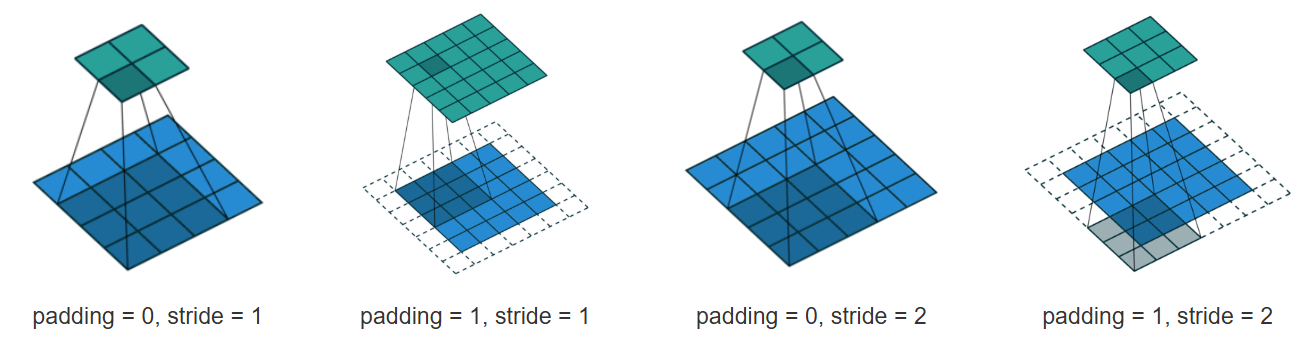
\includegraphics[width=1\textwidth,height=1\textheight,keepaspectratio]{images/padding-stride.png}
    \end{figure}
\end{frame}